% !TeX program = xelatex
% Compile: xelatex thuyetminh_de_tai_en.tex && xelatex thuyetminh_de_tai_en.tex
% English version of the Student Scientific Research Project Proposal
% (structure follows the official template of the University of Information
% Technology, VNU-HCM: A. General Information, B. Research Description)
\documentclass[a4paper,12pt]{article}

\usepackage{fontspec}
\setmainfont{Noto Serif}
\setsansfont{Noto Sans}

\usepackage[a4paper,margin=2.3cm]{geometry}
\usepackage{amsmath,amssymb}
\usepackage{graphicx}
\usepackage{booktabs}
\usepackage{longtable}
\usepackage{array}
\usepackage{enumitem}
\usepackage{xcolor}
\usepackage{hyperref}
\hypersetup{
    colorlinks=true,
    linkcolor=blue!45!black,
    urlcolor=blue!45!black,
    citecolor=blue!45!black,
    pdftitle={Student Research Proposal -- SADGS Digital Twin},
    pdfauthor={Digital Twin GS}
}
\usepackage{titlesec}

\definecolor{hdblue}{RGB}{31,73,125}
\titleformat{\section}{\normalfont\large\bfseries\color{hdblue}}{\thesection.}{0.5em}{}
\titleformat{\subsection}{\normalfont\normalsize\bfseries\color{hdblue}}{\thesubsection}{0.5em}{}

\setlength{\parindent}{0pt}
\setlength{\parskip}{5pt}

\begin{document}

% ---------------------------------------------------------------------
% Administrative header
% ---------------------------------------------------------------------
\begin{minipage}[t]{0.68\textwidth}
\centering
\textsc{VIETNAM NATIONAL UNIVERSITY , HO CHI MINH CITY}\\
\textbf{INTERNATIONAL UNIVERSITY}
\end{minipage}
\hfill
\begin{minipage}[t]{0.28\textwidth}
\small

\end{minipage}

\vspace{0.6cm}
\begin{center}
{\LARGE\bfseries PROJECT PROPOSAL}\\[2pt]
\end{center}

\vspace{0.4cm}
\section*{A. GENERAL INFORMATION}
\vspace{-0.3cm}

\subsection*{A1. Project Title}
\begin{itemize}[leftmargin=1.2em]

\textbf{"High-Fidelity Digital Twin Reconstruction of Base Transceiver Stations: Enhancing Vanilla 3DGS for Accelerated Training and Superior Rendering"}
\end{itemize}

\subsection*{A2. Duration}
3 months .

\subsection*{A3. Principal Investigator}
\begin{tabular}{@{}ll@{}}
Full name: & Lê Anh Kiệt \\
Student ID: & ITCSIU24047 \\
University: & International University -- Vietnam National University Ho Chi Minh City \\

\end{tabular}

\subsection*{A4. Project Members (including the Principal Investigator)}
\begin{longtable}{@{}p{0.6cm} p{4.2cm} p{3cm} p{5cm}@{}}
\toprule
\textbf{No.} & \textbf{Full name} & \textbf{Student ID} & \textbf{University / School} \\
\midrule
\endhead
1 & Lê Anh Kiệt & ITCSIU24047 & International University -- VNU-HCM \\
\bottomrule
\end{longtable}

\newpage
\section*{B. RESEARCH DESCRIPTION}

\subsection*{B1. Introduction}

3D Gaussian Splatting (3DGS) enables the reconstruction of 3D models of BTS towers directly from
on-site photographs, supporting the creation of digital twins for remote monitoring and
maintenance. However, the training process of vanilla 3DGS is still slow and generates many
redundant Gaussians on flat surfaces (the tower body, the ground), while not focusing enough on
complex structural details such as antennas, steel frames, and mechanical components on the
tower. This reduces efficiency when many BTS sites need to be reconstructed quickly over a wide
area.

This project surveys and verifies several 3DGS optimization techniques (structure-guided
densification, smart pruning, faster optimization), then combines the most effective techniques
into a single pipeline for BTS towers that trains faster and renders with higher fidelity than
vanilla 3DGS.

\begin{figure}[h]
\centering
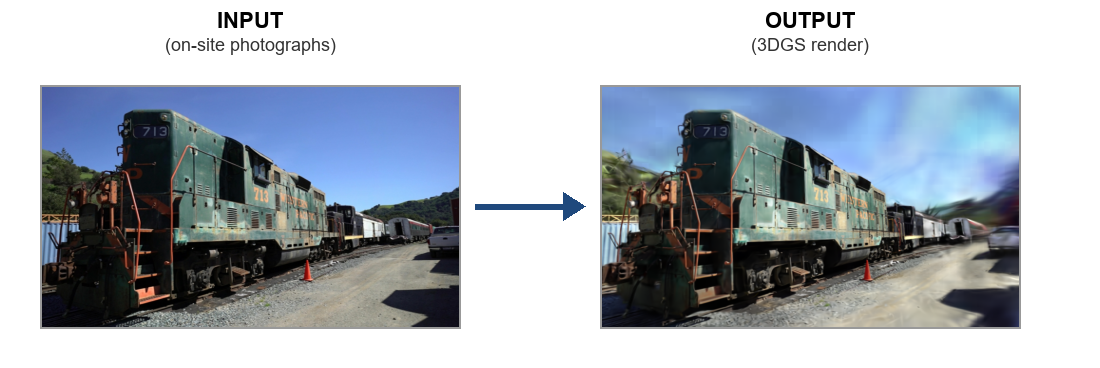
\includegraphics[width=0.9\textwidth]{figures/input_output_3dgs.png}
\caption{3DGS pipeline overview: a set of on-site photographs (input) is used to train a set of
3D Gaussians, which are then rendered into novel-view images (output).}
\end{figure}

\subsection*{B2. Objectives and Research Content}
\begin{itemize}[leftmargin=1.2em]
\item Study the original 3DGS pipeline and its training/density-control bottlenecks as the
baseline.
\item Survey multiple published techniques for faster training and better densification, and
verify each one against its own source code.
\item Select and combine the most effective techniques into one optimized pipeline for BTS
digital-twin reconstruction.
\item Benchmark the combined pipeline against vanilla 3DGS using PSNR, SSIM, LPIPS, Gaussian
count, training time, and memory use.
\end{itemize}

\subsection*{B3. Expected Results}
\begin{itemize}[leftmargin=1.2em]
\item A short, verified report and slides comparing multiple 3DGS optimization techniques.
\item An optimized 3DGS pipeline for BTS digital twins, combining the best-performing techniques.
\item A real benchmark table comparing the optimized pipeline with vanilla 3DGS.
\end{itemize}



\end{document}
